% Regarding `oneside` (https://stackoverflow.com/a/8371473/630364):
%
% `oneside` removes the blank pages between chapters.
% "Note that this method make the margins of all the pages the same. In
% `twoside`, the margins are different for the odd and the even pages".
\documentclass[12pt, letterpaper, oneside]{book}

\usepackage{amsfonts}
\usepackage{amsmath}
\usepackage{amssymb}
\usepackage{csquotes}
\usepackage{float}
\usepackage[letterpaper, textwidth=7.5in, textheight=8in]{geometry}
\usepackage{hyperref}
\usepackage{parskip}
\usepackage{pseudocode}
\usepackage{tikz}
\usetikzlibrary{shapes.geometric}
\usepackage{titlesec}
\usepackage{xcolor}

\hypersetup{
  colorlinks=true,
  linkcolor=blue,
  filecolor=magenta,
  urlcolor=blue,
}

\setcounter{secnumdepth}{4}

\title{
  Notes on \textit{Stanford: CS103: Mathematical Foundations of Computing}
}
\author{Yaobin Wen}
\date{July 2023}

\begin{document}

\maketitle
\tableofcontents

\chapter*{Overview}
\addcontentsline{toc}{chapter}{Overview}

This document contains my study notes of the Stanford course \textit{CS103:
  Mathematical Foundations of Computing}. I use it for a few purposes:

\begin{enumerate}
  \item As a reference to quickly refresh my memory on the subjects.
  \item Keep the notes to help me understand the text that is not obvious for
        me to comprehend.
\end{enumerate}

% =============================================================================
%
% Set Theory
%
% =============================================================================

\chapter{Set Theory}

% =============================================================================
\section{Is 0 a natural number?}
% =============================================================================

Is $0$ a natural number? Does $\mathbb{N}$ include $0$?

There is no ``yes'' or ``no'' answer to these questions. Take a look at
\href{https://math.stackexchange.com/q/283/665777}{this question} and you will
find people all over the world have all kinds of understanding such as:
\begin{itemize}
  \item $0$ is definitely \textbf{NOT} a natural number and does not belong to
        $\mathbb{N}$.
  \item There are two conventions: In one convention, $0$ is not a natural
        number; in another convention, $0$ is a natural number.
  \item Natural numbers include 0; those positive integers are called ``whole
        numbers'':
        \begin{displayquote}
          I see plenty of both these days, but when I was at school and at
          university, I almost only saw them defined to be {0, 1, ..}. The elements
          of {1, 2, ..} were called the whole numbers in my school days.
        \end{displayquote}
  \item Natural numbers don't include 0; whole numbers, denoted as $\mathbb{W}$,
        include $0$.
  \item $\mathbb{N}$ includes 0; $\mathbb{N^+}$ is all the positive integers so
        it doesn't include 0.
  \item yadda yadda yadda...
\end{itemize}

So I don't think it makes sense to argue whether $0$ is a natural number or not.
We just need to define it clearly and move on.

In CS103, $\mathbb{N}$ represents the natural numbers that \textbf{include} $0$.
But if you read 18.100A, you'll see in that course, $\mathbb{N}$ does not
include $0$.

That's fine. The world is still in peace. So in this note, I will respect the
choice of CS103 and treat $\mathbb{N}$ as the set of all the non-negative
integers, i.e., \[\{0, 1, 2, 3, \ldots\}\].

% =============================================================================
\section{Introduction to Set Theory}
% =============================================================================

This first lecture introduces set theory. Because I have learned them in MIT
OCW 18.100A Real Analysis, I won't repeat the notes again because they can be
found in the notes for that course. Here, I will just mention a few points that
are not covered in 18.100A.

\begin{itemize}
  \item Set difference: 18.100A uses $A \setminus B$ to denote ``A minus B''.
        CS103 says $A - B$ is also used.
  \item \textbf{Symmetric difference}: $A \bigtriangleup B = (A \setminus B)
          \cup (B \setminus A) = (A \cup B) \setminus (A \cap B)$. For example, if
        $A = \{1, 2, 3\}$ and $B = \{3, 4, 5\}$, then $A \bigtriangleup B = \{1, 2,
          4, 5\}$. \colorbox{red}{\textcolor{yellow}{TODO:}} Add a Venn diagram.
\end{itemize}

% =============================================================================
\section{Cardinality}
% =============================================================================

% ******************************
\subsection{$|\mathbb{N}|$ and $|\mathbb{Z}|$}
% ******************************

I've already learned that $|\mathbb{Z}|$ and the set of all the even (or odd)
numbers have the same cardinality, but in CS103 I just learned $|\mathbb{N}| =
  |\mathbb{Z}|$. The bijection (see 18.100A) between $\mathbb{N}$ and $\mathbb{Z}$
is created in the following way:
\begin{itemize}
  \item All the non-negative even numbers (including $0$) in $\mathbb{N}$ are
        matched to one non-negative integers in $\mathbb{Z}$.
  \item All the non-negative odd numbers in $\mathbb{N}$ are matched to one
        negative integers in $\mathbb{Z}$.
\end{itemize}

Visualized, this can be shown as:
\begin{itemize}
  \item $0 \longleftrightarrow 0$
  \item $1 \longleftrightarrow -1$
  \item $2 \longleftrightarrow 1$
  \item $3 \longleftrightarrow -2$
  \item $4 \longleftrightarrow 2$
  \item $5 \longleftrightarrow -3$
  \item $6 \longleftrightarrow 3$
  \item $7 \longleftrightarrow -4$
  \item $8 \longleftrightarrow 4$
  \item etc.
\end{itemize}

In general, the bijection $f: \mathbb{N} \rightarrow \mathbb{Z}$ is defined as:

\[
  f(n) = \begin{cases}
    n / 2,        & if \ MOD(n) = 0 \\
    (-n - 1) / 2, & if \ MOD(n) = 1
  \end{cases}
\]

where $n \in \mathbb{N}$.

% ******************************
\subsection{Cantor's diagonalization proof}
% ******************************

\href{https://en.wikipedia.org/wiki/Cantor%27s_diagonal_argument}{Cantor's
  diagonalization proof} is used to prove $|S| < |\mathcal{P}(S)|$.

% ******************************
\subsection{$|Programs| < |Problems|$}
% ******************************

This is the most interesting conclusion I've seen in this lecture. The proof
process can be summarized as follows:
\begin{itemize}
  \item Because every valid computer program is essentially a string, but not
        every string is a valid program, we can see \[|Program| \leq |Strings|\].
  \item The problems in the world may or may not deal with sets of strings.
        Suppose $S$ denotes a set of strings, so one kind of problems is: Given a
        string $s$, determine whether $s \in S$. For example:
        \begin{itemize}
          \item Suppose S = \{ ``a'', ``b'', ``c'', $\ldots$, ``z'' \}, then the
                problem can be: Given a string $s$, determine whether $s$ is an English
                letter.
          \item Suppose S = \{ ``0'', ``1'', ``2'', ``3'', $\ldots$ \}, then the
                problem can be: Given a string $s$, determine whether $s$ represents a
                natural number.
        \end{itemize}
  \item Not to mention that other kinds of problems can exist and may not be
        converted to problems that deal with sets of strings.
  \item The conclusion is: $|Sets\ of\ strings| \leq |Problems|$. They could be
        equal, if all the problems can be converted to problems that deal with sets
        of strings.
  \item Therefore:
        \[|Program| \leq |Strings| < |Sets\ of\ strings| \leq |Problems|\]
\end{itemize}

% =============================================================================
%
% Mathematical Proofs
%
% =============================================================================

\chapter{Mathematical Proofs}

\begin{enumerate}
  \item $\blacksquare$ means ``end of proof''.
  \item Use the ``mugga mugga'' test to verify if the proof is written in valid
        sentences: Replace all the mathematical notation with ``mugga mugga''. What
        comes back should still be a valid sentence.
  \item The section ``Proofs as a Dialog'' is interesting: It says the variables
        used in a proof can be divided into three categories:
        \begin{enumerate}
          \item Proof writer picks. Example: ``Let r = n + 1''
          \item Proof reader picks. Example: ``Consider some $n \in \mathbb{N}$''
          \item Neither picks: The variable's value is determined by some laws or
                definition. Example: ``If $n$ is even, there exists a $k$ so that $n =
                  2k$''. In this case, if the reader chooses an arbitrary even number $n$,
                the corresponding $k$'s value is not chosen by either the reader or the
                writer but by the definition of ``even''.
        \end{enumerate}
        Knowing which variables are picked by whom can help verify if the proof
        makes sense. Don't change the variables you (the proof writer) don't own.
\end{enumerate}

% =============================================================================
%
% Indirect Proofs
%
% =============================================================================

\chapter{Indirect Proofs}

% =============================================================================
\section{Implication}
% =============================================================================

An implication can be denoted as $p \rightarrow q$:
\begin{enumerate}
  \item In mathematics, implication is directional.
  \item In mathematics, implications only say something about the consequent
        when the antecedent is true.
  \item In mathematics, implication says nothing about causality.
\end{enumerate}

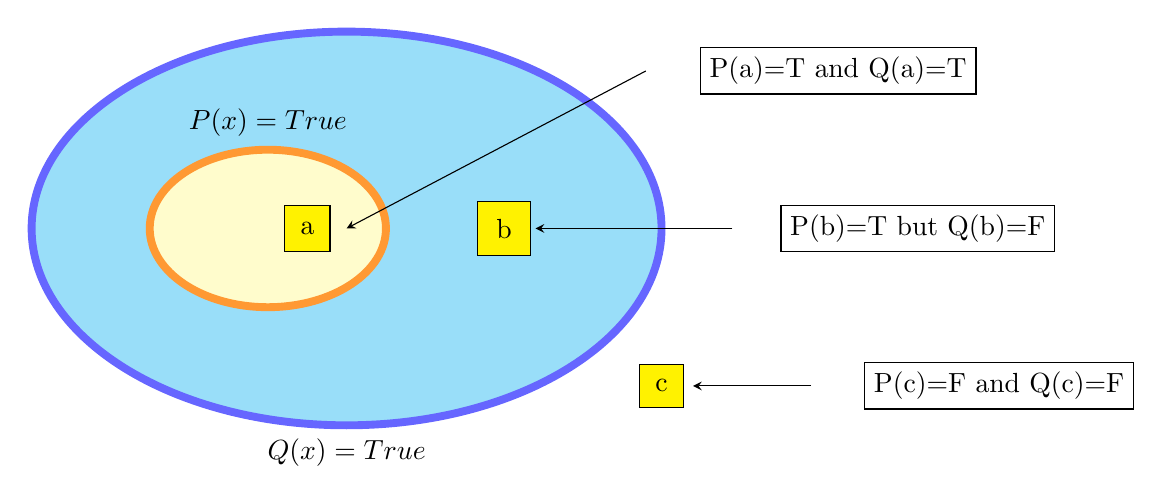
\begin{tikzpicture}
  % Set Q, the enclosing set.
  \node [ellipse,
    draw=blue!60,
    fill=cyan!40,
    line width=1mm,
    minimum width=8cm,
    minimum height=5cm,
    label={-90:$Q(x)=True$}] (Q) at (0,0) {};

  % Set P, the enclosed set.
  \node [ellipse,
    draw=orange!80,
    fill=yellow!20,
    line width=1mm,
    minimum width=3cm,
    minimum height=2cm,
    label={$P(x)=True$}] (P) at (-1,0) {};

  % Element a where P(a) = True and Q(a) = True
  \node [
    regular polygon,
    draw,
    regular polygon sides=4,
    minimum size=0.5cm,
    fill=yellow] (a) at (-0.5,0) {a};
  \node[
    draw=black,
    left, black, fill=white] at (8,2) {P(a)=T and Q(a)=T};
  \draw [-stealth] (3.8,2) -- (0,0);

  % Element b where P(b) = True but Q(b) = False
  \node [
    regular polygon,
    draw,
    regular polygon sides=4,
    minimum size=0.5cm,
    fill=yellow] (b) at (2,0) {b};
  \node[
    draw=black,
    left, black, fill=white] at (9,0) {P(b)=T but Q(b)=F};
  \draw [-stealth] (4.9,0) -- (2.4,0);

  % Element c where P(c) = True and Q(c) = True
  \node [
    regular polygon,
    draw,
    regular polygon sides=4,
    minimum size=0.5cm,
    fill=yellow] (c) at (4,-2) {c};
  \node[
    draw=black,
    left, black, fill=white] at (10,-2) {P(c)=F and Q(c)=F};
  \draw [-stealth] (5.9,-2) -- (4.4,-2);
\end{tikzpicture}

% =============================================================================
\section{Negation}
% =============================================================================

The negation of the \textbf{universal} statement is the \textbf{existential}
statement:
\begin{enumerate}
  \item ``Every P is a Q'' $\rightarrow$ ``There is a P that is not a Q''
  \item ``$\forall x: P(x)=True$'' $\rightarrow$ ``$\exists x: P(x)=False$''
\end{enumerate}

The negation of the \textbf{existential} statement is the \textbf{universal}
statement:
\begin{enumerate}
  \item ``There exists a P that is a Q'' $\rightarrow$ ``Every P is not a Q''
  \item ``$\exists x: P(x)=True$'' $\rightarrow$ ``$\forall x: P(x)=False$''
\end{enumerate}

% -----------------------------------------------------------------------------
\subsection{Negate an implication}
% -----------------------------------------------------------------------------

How to negate the implication:

\begin{displayquote}
  If Nanni pays money to Ea-Nasir, then Ea-Nasir will give Nanni quality copper
  ingots.
\end{displayquote}

An implication should be viewed as in the form as follows:

\begin{displayquote}
  For any x, if P(x) is true, then Q(x) is also true.
\end{displayquote}

Therefore the implication above should be re-interpretted as follows:

\begin{displayquote}
  For any time when Nanni pays money to Ea-Nasir, then Ea-Nasir will give Nanni
  quality copper ingots.
\end{displayquote}

So the negation of the concerned implication is:

\begin{displayquote}
  There are times when Nanni pays money to Ea-Nasir, then Ea-Nasir does not
  give Nanni quality copper ingots.
\end{displayquote}

% =============================================================================
\section{Proof by Contrapositive}
% =============================================================================

The contrapositive of the implication

\begin{displayquote}
  If \textbf{\textcolor{teal}{P is true}}, then \textbf{\textcolor{violet}{Q is
      true}}
\end{displayquote}

is the implication

\begin{displayquote}
  If \textbf{\textcolor{violet}{Q is false}}, then \textbf{\textcolor{teal}{P
      is false}}.
\end{displayquote}

They are \textbf{equivalent}.

To prove the original proposition, one can prove its contrapositive, hence
``proof by contrapositive''.

% =============================================================================
\section{Biconditionals}
% =============================================================================

Biconditionals are the ``if and only if''s, namely $p \Leftrightarrow q$.

To prove a biconditional, we must prove two directions: $p \Rightarrow q$ and
$q \Rightarrow p$.

% =============================================================================
\section{Proof by contradiction}
% =============================================================================

Example of how to write a proof by contradiction:

\begin{displayquote}
  Theorem: There is no largest set.

  Proof: \textbf{\textcolor{violet}{Assume for the sake of contradiction}} that
  \textbf{\textcolor{orange}{there is a largest set; call it $S$}}.

  (Steps to show the contradiction.)

  (Conclusion) \textbf{\textcolor{teal}{We've reached a contradiction, so our
      assumption must have been wrong. Therefore, there is no largest set.}}
  $\blacksquare$
\end{displayquote}

% =============================================================================
%
% Propositional Logic
%
% =============================================================================

\chapter{Propositional Logic}

% =============================================================================
\section{Proposition}
% =============================================================================

% ******************************
\subsection{Definition}
% ******************************

A \textbf{proposition} is a statement that is, by itself, either \textbf{true}
or \textbf{false}.
\begin{itemize}
  \item Commands are not propositions. Example: Open the door.
  \item Questions are not propositions. Example: What day is it today?
\end{itemize}

A \textbf{propositional variable}, usually a lower-case English letter such as
$p$, $q$, $r$, represents a proposition.

A \textbf{propositional connective} expresses how propositions are related.
Some of the connectives are:
\begin{itemize}
  \item $\lnot p$: ``NOT p''; logical negation.
  \item $p \land q$: ``p AND q''; logical conjunction.
  \item $p \lor q$: ``p OR q''; logical disjunction (inclusive). ``inclusive''
        means $p$ and $q$ can be $true$ at the same time, while ``exclusive or''
        means $p$ and $q$ cannot be $true$ at the same time.
  \item $p \rightarrow q$: ``p implies q''; material condition.
  \item $p \leftrightarrow q$: ``p if and only if q'', which also means ``(p
        implies q) AND (q implies p)''.
  \item $\top$: ``(always) true'' ($\top$ looks like a upper-case ``T'' that
        can represent ``True''.)
  \item $\bot$: ``(always) false''
\end{itemize}

% ******************************
\subsection{Example of using $\top$ and $\bot$}
% ******************************

$\bot$ can be used to describe how proof by contradiction works. Suppose that
you want to prove $p$ is $true$ using proof by contradiction. The usual steps
are as follows:
\begin{enumerate}
  \item Assume $p$ is $false$.
  \item Derive a conclusion that is known as $false$ (e.g., ``3 is even'').
  \item Conclude that $p$ is $true$.
\end{enumerate}

Described in propositional logic, it is
\[
  (\lnot p \rightarrow \bot) \rightarrow p
\].

% ******************************
\subsection{Logical operator precedence}\label{logical_operator_precedence}
% ******************************

All the logical operators are \textbf{right-associative}.

In the order of highest to lowest, they are:
\begin{enumerate}
  \item $\lnot$
  \item $\land$
  \item $\lor$
  \item $\rightarrow$
  \item $\leftrightarrow$
\end{enumerate}

For example, the statement
\[
  \lnot x \rightarrow y \lor z \rightarrow x \lor y \and z
\]
can be grouped as follows:
\[
  (\lnot x) \rightarrow ((y \lor z) \rightarrow (x \lor (y \and z)))
\]

% ******************************
\subsection{Truth table}
% ******************************

I have already learned the truth tables for $\lnot$, $\land$, and $\lor$. What
is surprising to me is the truth table for $\rightarrow$:

\begin{table}[H]
  \centering
  \begin{tabular}{|c|c|c|ll}
    \cline{1-3}
    p & q & $p \rightarrow q$ &  & \\ [1ex] \cline{1-3}
    F & F & T                 &  & \\ [0.5ex] \cline{1-3}
    F & T & T                 &  & \\ [0.5ex] \cline{1-3}
    T & F & F                 &  & \\ [0.5ex] \cline{1-3}
    T & T & T                 &  & \\ [0.5ex] \cline{1-3}
  \end{tabular}
  \caption{Truth table for $p \rightarrow q$}
\end{table}

The first two lines are the most confusing to many people, and there are many
questions about them. Here are some of them:
\begin{itemize}
  \item \href{https://philosophy.stackexchange.com/q/26719/44172}{Shouldn't statements be considered equivalent based on their meaning rather than truth tables?}
  \item \href{https://philosophy.stackexchange.com/q/34082/44172}{Why are conditionals with false antecedents considered true?}
  \item \href{https://math.stackexchange.com/q/3098664/665777}{How Implication or Material/Concrete Conditional works when the antecedent is false and the consequent is true}
  \item \href{https://math.stackexchange.com/q/70736/665777}{In classical logic, why is ($p \rightarrow q$) True if p is False and q is True?}
  \item And many more...
\end{itemize}

I read some of the posts and then decided to stop because this looks like a
deep rabbit hole. For now, it is better to just accept the truth table and move
on. But to help understand them a little bit:
\begin{itemize}
  \item $p \rightarrow q \equiv \lnot p \lor q \equiv \lnot (p \land \lnot q)$.
  \item $\lnot (p \rightarrow q) \equiv p \land \lnot q$.
  \item It's helpful to think about ``Ex falso sequitur quodlibet'' which means
        ``from what is false any assertion validly follows''.
\end{itemize}

\colorbox{red}{\textcolor{yellow}{TODO:}} Figure out why $F \rightarrow F$ is
$T$ and $F \rightarrow T$ is $T$. Or figure out why $p \rightarrow q$ is
equivalent to $\lnot p \lor q$.

Here is the truth table for $p \leftrightarrow q$:

\begin{table}[H]
  \centering
  \begin{tabular}{|c|c|c|ll}
    \cline{1-3}
    p & q & $p \leftrightarrow q$ &  & \\ [1ex] \cline{1-3}
    F & F & T                     &  & \\ [0.5ex] \cline{1-3}
    F & T & F                     &  & \\ [0.5ex] \cline{1-3}
    T & F & F                     &  & \\ [0.5ex] \cline{1-3}
    T & T & T                     &  & \\ [0.5ex] \cline{1-3}
  \end{tabular}
  \caption{Truth table for $p \rightarrow q$}
\end{table}

% ------------------------------
\subsubsection{Vacuously true; trivially true}
% ------------------------------

An implication with a false antecedent is called \textbf{vacuously true}, such
as $F \rightarrow F: T$ and $F \rightarrow T: T$.

An implication with a true consequent is called \textbf{trivially true}, such
as $F \rightarrow T: T$ and $T \rightarrow T: T$.

Note that the implication $F \rightarrow F: T$ is \textbf{both vacuous and
  trivial}.

Note that the implication $T \rightarrow F: F$ is \textbf{neither of them}.

% ******************************
\subsection{de Morgan's Laws}
% ******************************

\begin{itemize}
  \item $\lnot (p \land q) \equiv \lnot p \lor \lnot q$
  \item $\lnot (p \lor q) \equiv \lnot p \land \lnot q$
\end{itemize}

% =============================================================================
%
% First-Order Logic
%
% =============================================================================

\chapter{First-Order Logic}

% =============================================================================
\section{What is First-Order Logic?}
% =============================================================================

First-order logic:
\begin{enumerate}
  \item It is a a logical system for reasoning about properties of objects.
        There are two kinds of objects:
        \begin{enumerate}
          \item \textbf{Constants}: A symbol that refers to a specific object. For
                example, ``You'', ``Me'', ``EastAtlanta'', ``137''. Note that
                numbers such as ``137'' are \textbf{not} built in to first-order logic.
                They are just constant symbols like ``You'' and ``Me''.
          \item \textbf{Variables}: A symbol that serves as a placeholder to
                represent any object in a particular set. Usually this is used when
                \textbf{quantifiers} is used (because when quantifiers are used, we
                don't specify just one specific object, so we need a symbol to
                represent any of such objects we are referring to).
        \end{enumerate}
  \item It is built upon propositional logic.
  \item It uses the following three devices to describe more complex logic:
        \begin{enumerate}
          \item \textbf{predicates}: Describe \textbf{properties} of objects. It
                can take one or more objects as input and turn them into a proposition
                which is evaluated as $true$ or $false$.
                \begin{enumerate}
                  \item Binary predicates are sometimes written in \textbf{infix
                          notation}. For example, instead of writing ``$<(x, 8)$'', it's
                        more natural to write ``$x < 8$''.
                \end{enumerate}
          \item \textbf{functions}: Map objects to objects.
          \item \textbf{quantifiers}: Describe the quantities of objects, mainly
                two cases: ``for all objects'' and ``for some objects''.
        \end{enumerate}
  \item Examples:
        \begin{enumerate}
          \item $Likes(You, Eggs) \land Likes(You, Tomato) \rightarrow
                  Likes(You, Shakshuka)$
          \item $In(MyHeart, Havana) \land TookBackTo(Him, Me, EastAtlanta)$
        \end{enumerate}
\end{enumerate}

% =============================================================================
\section{Equality}
% =============================================================================

\begin{enumerate}
  \item The predicates ``$=$'' and ``$\neq$'' indicate whether two
        \textbf{objects} are equal or not.
  \item ``$\leftrightarrow $'' indicates that two \textbf{propositions} are
        equal. Note that ``$\leftrightarrow $'' is not a predicate because
        predicates are applied to objects to describe the objects' properties, but
        ``$\leftrightarrow $'' is applied to propositions to describe their logical
        relations.
\end{enumerate}

% =============================================================================
\section{Type-Checking Table}
% =============================================================================

\begin{table}[H]
  \centering
  \begin{tabular}{|l|l|l|}
    \hline
    \textbf{}            & \textbf{...operate on..} & \textbf{...produce} \\ [1ex] \hline
    \textbf{Connectives} & propositions             & a proposition       \\ [1ex] \hline
    \textbf{Predicates}  & objects                  & a proposition       \\ [1ex] \hline
    \textbf{Functions}   & objects                  & an object           \\ [1ex] \hline
  \end{tabular}
  \caption{Type-Checking Table}
  \label{FOL_type_checking_table}
\end{table}

% =============================================================================
\section{Existential and Universal Quantifiers}
% =============================================================================

% ******************************
\subsection{General form}
% ******************************

The general form of using the quantifiers is as follows:
\begin{enumerate}
  \item $\exists x. PROPERTY(x)$: Some $x$ has the property ``PROPERTY''.
  \item $\forall x. PROPERTY(x)$: All $x$ has the property ``PROPERTY''.
\end{enumerate}

To describe the set that $x$ belongs to, use the following forms:
\begin{enumerate}
  \item $\exists x. (x \in X \rightarrow PROPERTY(x))$
  \item $\forall x. (x \in X \rightarrow PROPERTY(x))$
\end{enumerate}

For example, ``For any natural number $n$, $n$ is even if and only if $n^2$ is
even'' can be translated into
\[
  \forall n. (n \in \mathbb{N} \rightarrow (Even(n) \leftrightarrow Even(n^2)))
\]

% ******************************
\subsection{Edge cases}
% ******************************

I'm familiar with the existential quantifier ``$\exists$'' and the universal
quantifier ``$\forall$'', but I didn't think about the two edge cases before:
\begin{enumerate}
  \item $\exists x. (x \in \emptyset \rightarrow PROPERTY(x) = \bot)$, i.e.,
        existentially-quantified statements are always \textbf{false} in an empty
        world because \textbf{nothing exists}.
  \item $\forall x. (x \in \emptyset \rightarrow PROPERTY(x) = \top)$, i.e.,
        universally-quantified statements are said to be \textbf{vacuously true} in
        an empty world.
\end{enumerate}

% ******************************
\subsection{Association}
% ******************************

The variable is scoped just to the statement being quantified. For example:
\[(\exists x. BIGGER(A, x)) \land (\exists y. SMALLER(y, B))\]

\begin{enumerate}
  \item $x$ is only applicable to ``BIGGER''.
  \item $y$ is only applicable to ``SMALLER''.
\end{enumerate}

% ******************************
\subsection{Precedence}
% ******************************

Quantifiers have precedence just below ``$\lnot$''. See
\ref{logical_operator_precedence}.

Therefore, the statement \[\exists x. P(x) \land R(x) \land Q(x)\] is parsed as
\[(\exists x. P(x)) \land R(x) \land Q(x)\] which is \textbf{syntactically
  invalid} because the variable $x$ is out of scope for $R$ and $Q$.



% =============================================================================
%
% Functions
%
% =============================================================================

\chapter{Functions}

 (TODO)

% =============================================================================
%
% Graphs
%
% =============================================================================

\chapter{Graphs}

 (TODO)

% =============================================================================
%
% Mathematical Induction
%
% =============================================================================

\chapter{Mathematical Induction}

 (TODO)

% =============================================================================
%
% Finite Automata
%
% =============================================================================

\chapter{Finite Automata}

% =============================================================================
\section{Computability Theory}
% =============================================================================

\textbf{Two key questions}: How can we prove what computers can and can't do...
\begin{enumerate}
  \item ... so that our results are still true in 20 years?
  \item ... without multi-hundred page proofs?
\end{enumerate}

% ******************************
\subsection{Finite Automata: Modeling Finite Computation}
% ******************************

\colorbox{lime}{\textbf{NOTE(ywen)}}: The automata seem to be different from the ``state machines'' I have understood
so far. The ``state machines'' I've been using are those whose every state is an ``accepting state'' (see below for the
meaning of an ``accepting state''), but an automaton may have accepting states (which the automaton returns ``Yes'' to
indicate the acceptance) and rejecting states (which the automaton returns ``No'' to indicate the rejection). In other
words, the ``state machines'' I've been using all the time are a subset of automata.

Slide 42 says:
\begin{displayquote}
  As a simplifying assumption, we'll assume that we just need to get a single
  bit of output. That is, our machines will just say \textbf{YES} or
  \textbf{NO}.
\end{displayquote}

\colorbox{red}{\textcolor{yellow}{TODO:}} I need to learn how the
generalization happens.

Slide 44 introduces the following terms:
\begin{itemize}
  \item \textbf{accepting states}: \colorbox{red}{\textcolor{yellow}{TODO:}}
        How to determine if a state is an accepting state?
  \item \textbf{accepts}: If the device ends in an \textbf{accepting state}
        after seeing all the input, it \textbf{accepts} the input (says
        \textbf{YES}).
  \item \textbf{rejects}: If the device does not end in an \textbf{accepting
          state} after seeing all the input, it \textbf{rejects} the input (says
        \textbf{NO}).
\end{itemize}

Finite automata model computers where:
\begin{enumerate}
  \item memory is finite.
  \item the computation produces as YES/NO answer. (``YES/NO" is similar to
        ``True/False". In other words, given the input, an automaton outputs
        ``True/False", so an automaton can be viewed as a \textbf{predicate}. See
        ``first-order logic'' for the meaning of a ``predicate''.)
\end{enumerate}

% ******************************
\subsection{Finite Automata and Languages}
% ******************************

In order to define finite automata and their languages, we need to define ``languages'' first.

% ------------------------------
\subsubsection{Alphabet}
% ------------------------------

An \textbf{alphabet} is:
\begin{enumerate}
  \item a \textbf{finite}, \textbf{nonempty} set of symbols called \textbf{characters}.
  \item denoted by $\Sigma$.
\end{enumerate}

For example, $\Sigma = \{a, b\}$ is an alphabet over the characters ``a'' and ``b''.

% ------------------------------
\subsubsection{Strings}
% ------------------------------

A \textbf{string} over an alphabet $\Sigma$ is a \textbf{finite} sequence of characters drawn from $\Sigma$. The
\textbf{empty string} has no characters and is denoted $\epsilon$. The set of \textbf{all strings} composed from the
characters in $\Sigma$ is denoted $\Sigma^*$.

For example, some strings over $\Sigma = \{a, b\}$ are: ``a'', ``ababbabbbababba'', ``abbabbab''.

% ------------------------------
\subsubsection{Languages}
% ------------------------------

A \textbf{language}:
\begin{enumerate}
  \item is a set of \textbf{strings}.
  \item is a language over $\Sigma$ if it is a subset of $\Sigma^*$.
\end{enumerate}

% ------------------------------
\subsubsection{Finite Automata and Languages}
% ------------------------------

Let $A$ be an automaton that processes strings drawn from an alphabet $\Sigma$. The language of $A$, denoted
$\mathfrak{L}(A)$, is the set of strings over $\Sigma$ that $A$ accepts:

\[
  \mathfrak{L}(A) = \{ w \in \Sigma^* | A \ accepts \ w \}
\]

Here ``$A$ accepts $w$'' is the general form of the rule about $w$. In a particular example of automaton, it can be
``$w$ ends in the character $a$''.

% ------------------------------
\subsubsection{Summary}
% ------------------------------

\begin{enumerate}
  \item A \textbf{finite automaton} is a collection of \textbf{states} joined by \textbf{transitions}.
  \item Some state is designated as the \textbf{start state}.
  \item Some number of states are designated as \textbf{accepting states}. These accepting states make the automaton
        return ``Yes''.
  \item The automaton processes a string by beginning in the start state and following the indicated transitions.
  \item If the automaton ends in an accepting state, it \textbf{accepts} the input. Otherwise, the automaton
        \textbf{rejects} the input.
  \item The \textbf{language} of an automaton is the set of strings it accepts.
\end{enumerate}

% =============================================================================
%
% Regular Expression
%
% =============================================================================

\chapter{Regular Expression}

 (TODO)

% =============================================================================
%
% Nonregular Languages
%
% =============================================================================

\chapter{Nonregular Languages}

 (TODO)

% =============================================================================
%
% Context-Free Languages
%
% =============================================================================

\chapter{Context-Free Languages}

 (TODO)

% =============================================================================
%
% Turing Machines
%
% =============================================================================

\chapter{Turing Machines}

 (TODO)

% =============================================================================
%
% Unsolvable Problems
%
% =============================================================================

\chapter{Unsolvable Problems}

 (TODO)

% =============================================================================
%
% Complexity Theory and P vs NP
%
% =============================================================================

\chapter{Complexity Theory and P vs NP}

 (TODO)

\chapter*{References}
\addcontentsline{toc}{chapter}{References}

\begin{itemize}
  \item $[1]$ \href{https://web.stanford.edu/class/cs103/}{CS103: Mathematical Foundations of Computing}
\end{itemize}

\end{document}
